\documentclass{standalone}

\usepackage{tikz}
\usepackage{pgfplots}
\usetikzlibrary{calc, tikzmark, shapes, shapes.arrows, arrows, 3d, positioning}
\pgfplotsset{compat=1.17}

\begin{document}
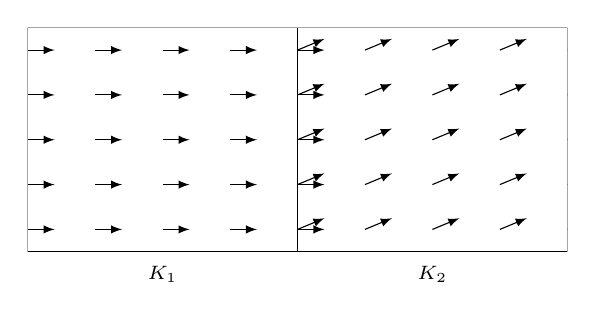
\begin{tikzpicture}
	\begin{axis}[view={0}{90}, xmax=2, ymin=-1, ymax=1, axis lines=none]
		\addplot3[black, quiver={u=1, v=0, scale arrows=0.1}, samples=5, -latex, domain=0:1, y domain=.1:.9] (x,y,0);
		\addplot3[black, quiver={u=1, v=.5, scale arrows=0.1}, samples=5, -latex, domain=1:2, y domain=.1:.9] (x,y,0);
		\draw (0,0,0) -- (2,0,0) -- (2,1,0) -- (0,1,0) -- (0,0,0); 
		\draw (1,0,0) -- (1,1,0); 

		\scriptsize
		\node at (.5,-.1,0) {$K_1$}; 
		\node at (1.5,-.1,0) {$K_2$}; 		
	\end{axis}
\end{tikzpicture}
\end{document}